\makeatletter
\def\input@path{{../}}
\makeatother
\documentclass[../master_thesis.tex]{subfiles}
\begin{document}
\chapter{Results}\label{chap:Results}
\section{Overview of Tests}
We divided the tests of this implementation into four main types, theoretical
correctness, parametrization, comparison and tests of the variational implementation.

In the tests of theoretical correctness we test if our implementation gives the
results to problems as expected. The tests for this were comparisons to
the energy of  \ce{Li^+} in an environment with dielectric constant $\epsinf = 2$
with the value we would get from the Born model. In the Born model the energy of a  %citation please
one atom ion in a solvent is the same as the energy of a point charge in the same solvent.
This energy is described as
\begin{equation}
  E_{ion} = -\frac{q^{2}}{8 \pi R_{cav}}\left(\frac{1}{\epso\\}-\frac{1}{\epsinf}\right)
\end{equation}
A second comparison with the Born model was done where we tested for the
following relation that should hold for a point charge
\begin{equation}
  \int \gamma_s = \frac{\epsinf - 1}{\epsinf} q
\end{equation}

The parametrization tests were done by changing one parameter at a time while
comparing this same change to Gaussian calculations with different basis sets.
First we only checked the dependency on the radius and how changing it would
affect the reaction field energy with respect to Gaussian calculations of the same
radii. We then compared Gaussian calculations of Radius $R$ against \mrchem
calculations of Radius $R+0.2$ in an attempt to see an improvement in the
results.
A second parametrization test was done with only \ce{Li^+}
where we changed the relative precision of the \mrchem calculations to see how
they affect the energy with respect to the Gaussian energies. This was also done
on different radii.

We then took 4 molecules that were tested by \cite{Chipman2002} and compared the
results from variation of radii against Gaussian results. The molecules used
were \ce{H_2O}, \ce{NO^+}, \ce{CN^-} and \ce{CH_3CONH_2}. These tests are classified into
single cavity tests and \ac{ABC} tests. Single cavity tests are performed in the
same manner as the parametrization tests where only the radius of the cavity was changed per
calculation. We did not shift the \mrchem calculation's cavity radius.

The \ac{ABC} tests consist of making spherical cavities centered on
each atom with radii equal to their center atom's Van der Waals radius. The Radii
used to represent the Van der Waals radii were the Bondi radii multiplied by a factor of
$1.2$ as outlined by \cite{Tomasi:1994wt}. These radii were later shifted in the same manner
as in the parametrization tests in order to see the effect of bigger spheres for each
atom.

As stated before in chapters \ref{chap:Solvent_effect} and \ref{chap:implementation}
a variational formulation of the Reaction field Problem was implemented in this thesis,
The tables in Appendix \ref{Datatables} show a row which is labeled "Variational",
though the variational implementation behaved in a irregular way. We will show
the Reaction energy plots for the variational implementation for both water
and \ce{Li^+} as those are the ones that had the most data points. We leave the
reader to evaluate the variational energies for the other molecules.


\section{Data}
\subsection{Theoretical correctness Tests}
\subsection{Parametrization Tests}\label{sec:paratests}
The data tables containing all results can be found in appendix \ref{Datatables}, following
tables will show a small sample so the reader can make have a understanding of
the tables shown there.
We first varied the Radius of the cavity for water and lithium. The following
table \ref{tab:rawwaterdata}  presents the data for the energy
calculations of \ce{H_2O} with the three first cavity radii as an example of the layout of the
tables.
These are the total  energy of the system including the solvent effect contributions.
The same type of tables were used for the rest of the systems.
\begin{table}[htbp]
  \caption{Total Energy Calculations example for Water in Water. Energy in Hartree and radii of the cavity in Bohr}
  \begin{center}
    \begin{tabular}{|l|r|r|r|r|}
      \hline
      Basis & $R =3.6$ & $R=3.7$ & $R=3.8$ & $\ldots$\\  \hline
      Cc-pVDZ & -7.6039e+01 & -7.6038e+01 & -7.6036e+01 & $\ldots$\\ \hline
      Cc-pVTZ & -7.6070e+01 & -7.6069e+01 & -7.6067e+01 & $\ldots$\\ \hline
      Cc-pVQZ & -7.6078e+01 & -7.6076e+01 & -7.6075e+01 & $\ldots$\\ \hline
      Cc-pV5Z & -7.6080e+01 & -7.6079e+01 & -7.6077e+01 & $\ldots$\\ \hline
      Aug-cc-pVDZ & -7.6054e+01 & -7.6053e+01 & -7.6052e+01 & $\ldots$\\ \hline
      Aug-cc-pVTZ & -7.6074e+01 & -7.6072e+01 & -7.6071e+01 & $\ldots$\\ \hline
      Aug-cc-pVQZ & -7.6079e+01 & -7.6077e+01 & -7.6076e+01 & $\ldots$\\ \hline
      Aug-cc-pV5Z & -7.6080e+01 & -7.6079e+01 & -7.6077e+01 & $\ldots$\\ \hline
      daug-cc-pVDZ & -7.6055e+01 & -7.6053e+01 & -7.6052e+01 & $\ldots$\\ \hline
      daug-cc-pVTZ & -7.6074e+01 & -7.6072e+01 & -7.6071e+01 & $\ldots$\\ \hline
      daug-cc-pVQZ & -7.6079e+01 & -7.6077e+01 & -7.6076e+01 & $\ldots$\\ \hline
      daug-cc-pV5Z & -7.6080e+01 & -7.6079e+01 & -7.6077e+01 & $\ldots$\\ \hline
      \mrchem & -7.6085E+01 & -7.6083E+01 & -7.6081E+01 & $\ldots$\\ \hline
    \end{tabular}
  \end{center}
  \label{tab:rawwaterdata}
\end{table}

In order to Calculate the Reaction field energy we took a gas phase calculation
of a basis set and subtracted it from the total energy calculated with the same
basis set. In \mrchem this was done using the same relative precision. The
following equation was used to calculate the Reaction field Energy $E_r$
\begin{equation}\label{eq:deltaer}
  E_r = E_{tot} - E_{vac}
\end{equation}
Examples of $E_r$ for the first three cavity radii for water obtained from the operation
in Equation \ref{eq:deltaer} can be seen in table \ref{tab:Erwatdata}

\begin{table}[htbp]
\caption{Reaction Field Energy Calculations example for Water in Water. Energy in Hartree and radii of the cavity in Bohr}
\begin{center}
\begin{tabular}{|l|r|r|r|r|}
\hline
Basis & 3.6 & 3.7 & 3.8 & $\ldots$\\ \hline
Cc-pVDZ & -1.2450E-02 & -1.0998E-02 & -9.7804E-03 & $\ldots$\\ \hline
Cc-pVTZ & -1.3097E-02 & -1.1545E-02 & -1.0243E-02 & $\ldots$\\ \hline
Cc-pVQZ & -1.3218E-02 & -1.1651E-02 & -1.0334E-02 & $\ldots$\\ \hline
Cc-pV5Z & -1.3284E-02 & -1.1713E-02 & -1.0393E-02 & $\ldots$\\ \hline
Aug-cc-pVDZ & -1.3190E-02 & -1.1634E-02 & -1.0328E-02 & $\ldots$\\ \hline
Aug-cc-pVTZ & -1.3238E-02 & -1.1670E-02 & -1.0353E-02 & $\ldots$\\ \hline
Aug-cc-pVQZ & -1.3221E-02 & -1.1655E-02 & -1.0338E-02 & $\ldots$\\ \hline
Aug-cc-pV5Z & -1.3223E-02 & -1.1655E-02 & -1.0337E-02 & $\ldots$\\ \hline
daug-cc-pVDZ & -1.3228E-02 & -1.1665E-02 & -1.0351E-02 & $\ldots$\\ \hline
daug-cc-pVTZ & -1.3243E-02 & -1.1675E-02 & -1.0357E-02 & $\ldots$\\ \hline
daug-cc-pVQZ & -1.3223E-02 & -1.1656E-02 & -1.0340E-02 & $\ldots$\\ \hline
daug-cc-pV5Z & -1.3224E-02 & -1.1655E-02 & -1.0337E-02 & $\ldots$\\ \hline
mrchem & -1.8036E-02 & -1.5494E-02 & -1.3437E-02 & $\ldots$\\ \hline
\end{tabular}
\end{center}
\label{tab:Erwatdata}
\end{table}


We now plot the data from the total energy and reaction energy tables for
both water and \ce{Li^+}.

The plots for the Reaction energy of water for
both the Gaussian and  \mrchem calculations can be seen in Figure \ref{fig:watEnergyplotsdaug}.
The same type of plots for \ce{Li^+} can be seen in Figure \ref{fig:lipEnergyplotsdaug}.
In both of these figure we are comparing the energy from \mrchem to sets of four
curves formed each of double, triple, quadruple and quintuple zeta Dunning's correlation
consistent \cite{doi:10.1063/1.456153} basis sets as implemented in Gaussian \cite{G09}.

While in this chapter we only look at double augmented basis, in Appendix \ref{Figures}
the reader can see this same comparison for augmented and standard basis sets for
both these tests and subsequent ones.


\begin{figure}[h!]
  \centering
    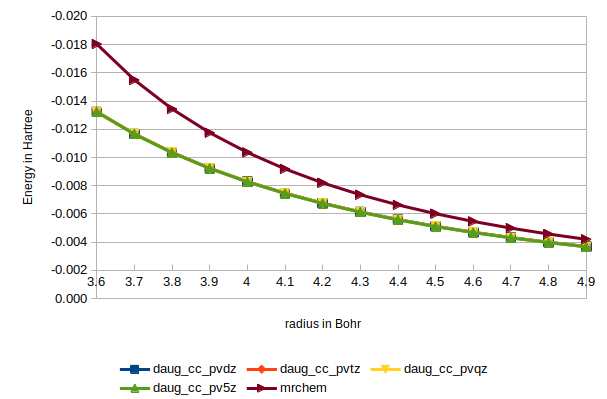
\includegraphics[width=0.75\linewidth]{img/Erdaugwat.png}
  \caption{Reaction field energy of Water in a water solution, calculated with relative precision $e-05$ in \mrchem and with double augmented basis sets in Gaussian}
  \label{fig:watEnergyplotsdaug}
\end{figure}

\begin{figure}[h!]
  \centering
    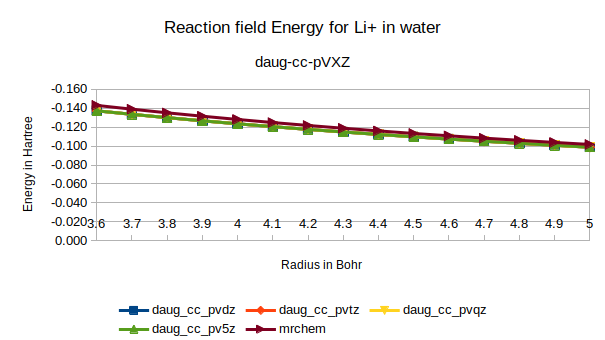
\includegraphics[width=0.75\linewidth]{img/Erdauglip.png}
  \caption{Reaction field energy of \ce{Li^+} in a water solution, calculated with relative precision $e-05$ in \mrchem  and with double augmented basis sets in Gaussian}
  \label{fig:lipEnergyplotsdaug}
\end{figure}

The \mrchem energy values $E_{Mrchem}$ for each radii were compared to the
corresponding values of each of the different basis set calculations in
Gaussian  $E_{Gaussian}^{basis}$ by finding the relative difference $d_r$
between them as
\begin{equation}\label{eq:reldiff}
  d_r = \frac{E_{Gaussian}^{basis} - E_{Mrchem}}{E_{Mrchem}}
\end{equation}
The operation in Equation \ref{eq:reldiff} was applied to both water and \ce{Li^+} for all the
substrate molecules, giving the following figures \ref{fig:watreldiffdaug} and \ref{fig:lipreldiffdaug}.


\begin{figure}[h!]
  \centering
    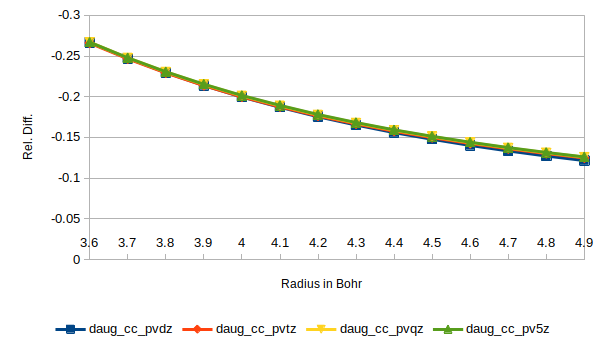
\includegraphics[width=\linewidth]{img/watdaugreldiff.png}
  \caption{Relative difference between the Reaction field energy of Water in a water solution calculated with with relative precision $e-05$ in \mrchem
   and with double augmented basis sets in Gaussian}
  \label{fig:watreldiffdaug}
\end{figure}

\begin{figure}[h!]
  \centering
  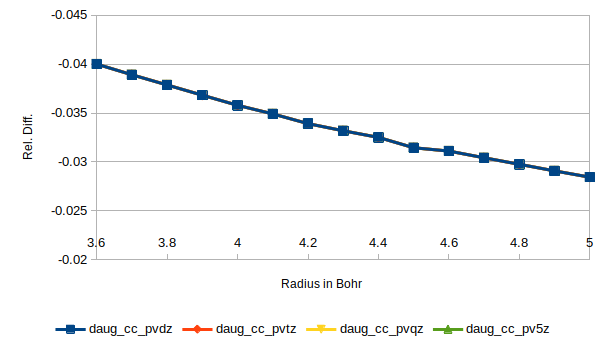
\includegraphics[width=\linewidth]{img/lipdaugreldiff.png}
  \caption{Relative difference between the Reaction field energy of\ce{Li^+} in a water solution calculated with relative precision $e-05$ in \mrchem
  and with double augmented basis sets in Gaussian}
  \label{fig:lipreldiffdaug}
\end{figure}


We then shifted the cavity radius of the \mrchem calculations for both water and
\ce{Li^+} so they were $0.2$ Bohr bigger and compared them to Gaussian calculations
with an unshifted Radius. The relative Difference plots for water and \ce{Li^+} can be seen
in Figures \ref{fig:watreldiff02daug} and \ref{fig:lipreldiff02daug} respectively.

\begin{figure}[h!]
  \centering
    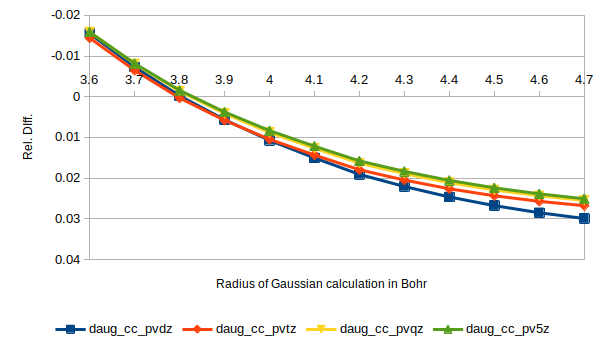
\includegraphics[width=\linewidth]{img/watdaugreldiff02.png}
  \caption{Relative difference between the Reaction field energy of Water in a water solution calculated with with relative precision $e-05$ in \mrchem
  and with double augmented basis sets in Gaussian}
  \label{fig:watreldiff02daug}
\end{figure}

\begin{figure}[h!]
  \centering
    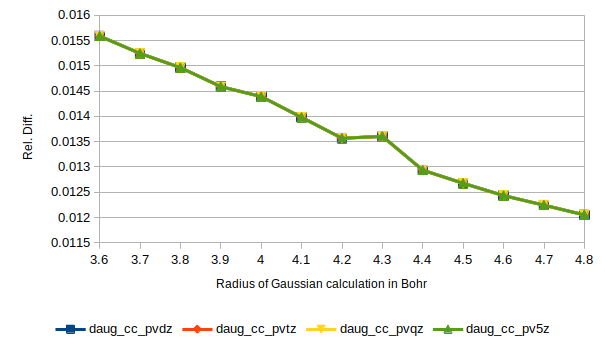
\includegraphics[width=\linewidth]{img/lipdaugreldiff02.png}
  \caption{Relative difference between the Reaction field energy of \ce{Li^+} in a water solution calculated with relative precision $e-05$ in \mrchem
  and with double augmented basis sets in Gaussian}
  \label{fig:lipreldiff02daug}
\end{figure}


Lastly we computed the reaction field energies of \ce{Li^+} with four different
relative precision; $1e-3, 1e-4, 1e-5,\  \text{and}\  1e-6$. We compared these
to the reaction field energies calculated with the most complete basis set:
\verb!daug-cc-pV5Z! as described in
\begin{equation}\label{eq:difgauss}
    d_r = \frac{E_{Li^+} - E_{Gaussian}}{E_{Gaussian}}
\end{equation}
Figure \ref{fig:lipprecreldef} shows the plots of the operation in Equation \ref{eq:difgauss} above.
First all of the relative differences plotted together, then the second one contains
only the results for relative precision $1e(-4), 1e(-5),\  \text{and}\  1e(-6)$ since
the results with relative precision $1e(-3)$ are over five times larger than the other ones.

\begin{figure}[h!]
  \centering
  \begin{subfigure}[b]{0.75\linewidth}
    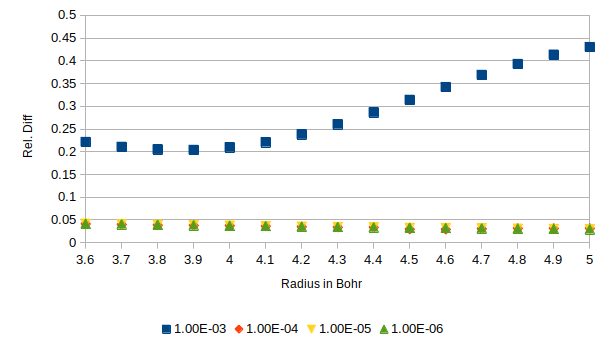
\includegraphics[width=\linewidth]{img/lipprecallreldiff.png}
  \end{subfigure}
  \begin{subfigure}[b]{0.75\linewidth}
    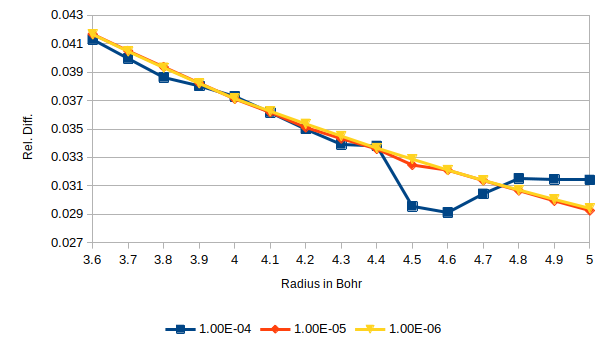
\includegraphics[width=\linewidth]{img/lipprecallreldiffexcl.png}
  \end{subfigure}
  \caption{Relative difference between the Reaction field energy of \ce{Li^+} in a water solution calculated with different relative precisions in \mrchem  and same calculations in Gaussian with daug-cc-pV5Z}
  \label{fig:lipprecreldef}
\end{figure}

\subsection{Comparison Tests}

These tests were divided into single cavity and \ac{ABC} tests. The single cavity
tests are the same type of tests performed on water in the previous sections. These
tests were applied to \ce{NO^+}  and \ce{CN^-}. We did not apply this test
on \ce{CH_3CONH_2} as the size of the molecule made the calculations in both Gaussian
and \mrchem extremely slow.

Following are figures \ref{fig:nopEnergyplotsdaug} and \ref{fig:cyanEnergyplotsdaug}
that show the energies of the \mrchem calculations plotted
against the energies from the Gaussian calculation for water, \ce{NO^+}, and
\ce{CN^-} respectively. Many of the \mrchem results for \ce{CN^-} and \ce{NO^+}
around the interval $(4.0, 4.5)$ diverged and finished or never finished
running due to divergence,  these results were therefore removed from the figures so as to facilitate
the visualization of the trends across the radii. The values which diverged but still
finished running can be viewed in section \ref{Datatables}.

\begin{figure}[h!]
  \centering
    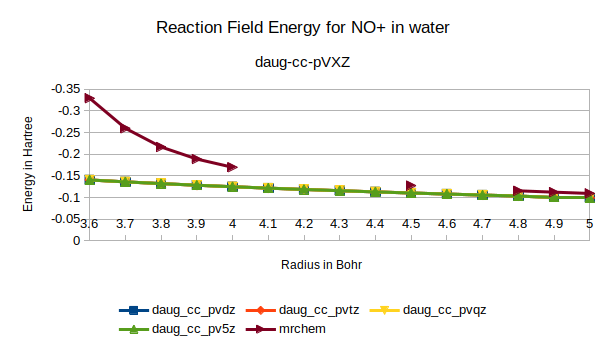
\includegraphics[width=\linewidth]{img/Erdaugnop.png}
  \caption[Energy plots for \ce{NO^+}]{Reaction field energy of \ce{NO^+} in a water solution, calculated with \mrchem
  and with double augmented basis sets in Gaussian}
  \label{fig:nopEnergyplotsdaug}
\end{figure}

\begin{figure}[h!]
  \centering
    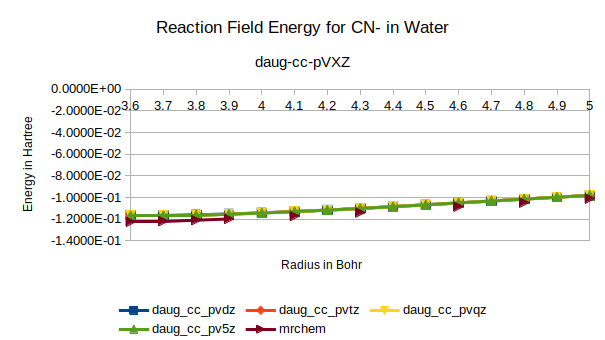
\includegraphics[width=\linewidth]{img/Erdaugcyan.png}
  \caption{Reaction field energy of \ce{CN^-} in a water solution, calculated with \mrchem
  and with different basis sets in Gaussian}
  \label{fig:cyanEnergyplotsdaug}
\end{figure}

The Figures \ref{fig:nopreldiffdaug} and \ref{fig:cyanreldiffdaug} show the relative
difference between the Gaussian and \mrchem results as shown in Equation \ref{eq:reldiff}

\begin{figure}[h!]
  \centering
    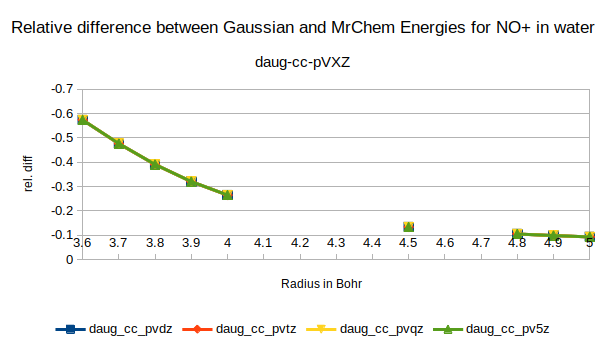
\includegraphics[width=\linewidth]{img/nopdaugreldiff.png}
    \caption{Relative difference between the Reaction field energy of \ce{NO^+} in a water solution calculated with \mrchem
  and with different basis sets in Gaussian}
  \label{fig:nopreldiffdaug}
\end{figure}

\begin{figure}[h!]
  \centering
    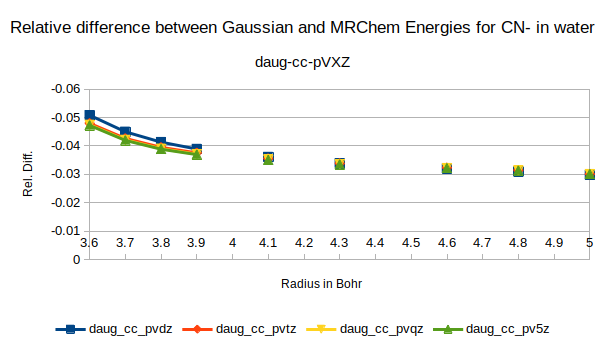
\includegraphics[width=\linewidth]{img/cyandaugreldiff.png}
  \caption{Relative difference between the Reaction field energy of \ce{CN^-} in a water solution calculated with \mrchem
  and with double augmented basis sets in Gaussian}
  \label{fig:cyanreldiffdaug}
\end{figure}


Since the \ac{ABC} tests were just two data points for each basis set and \newline\mrchem
we will present them in a tabulated manner. Here we did tests for \ce{CH_3CONH_2}, \ce{H_2O}, \ce{CN^-} and \ce{NO^+}
for both the Bondi Van der Waals radii and the same radii shifted by $0.2$ Bohr as was done previously.

Tables \ref{tab:watabcreldiff}, \ref{tab:nopabcreldiff}, \ref{tab:cyanabcreldiff}, \ref{tab:acetamidabcreldiff}
each show the relative difference for the \ac{ABC} and shifted \ac{ABC} tests
for \ce{H_20}, \ce{NO^+}, \ce{CN^-}, and \ce{CH_3CONH_2} respectively. The
total and  reaction field energy for each of these can be seen in appendix \ref{Datatables}.

The shifted \ac{ABC} did not converge for \ce{CN^-}, so a comparison between the two sets
of radii is not possible, we can still compare with the basis sets and see how it compared with
the rest of the single cavity values.

The \verb!daug-cc-pV5Z! Gaussian calculations for \ce{CH_3CONH_2} did not finish
after $72$ hours of running. We will therefore present the comparison to the other
basis sets and not include this one.

\begin{table}[htbp]
\caption{Relative difference between Gaussian and \mrchem results from \ac{ABC}  test for water}
\begin{tabular}{|l|r|r|}
\hline
Basis & \multicolumn{1}{l|}{Van der Waals Radii} & \multicolumn{1}{l|}{Van der Waals Radii $+ 0.2$ Bohr} \\ \hline
Cc-pVDZ & -0.150906543613475 & -0.141285964520019 \\ \hline
Cc-pVTZ & -0.128295351717095 & -0.119975293105413 \\ \hline
Cc-pVQZ & -0.12895264591432 & -0.120205694685673 \\ \hline
Cc-pV5Z & -0.129254059406516 & -0.119768698510995 \\ \hline
Aug-cc-pVDZ & -0.12913031667549 & -0.119600162056159 \\ \hline
Aug-cc-pVTZ & -0.134287756186553 & -0.124924550255723 \\ \hline
Aug-cc-pVQZ & -0.136838481699817 & -0.127632128628228 \\ \hline
Aug-cc-pV5Z & -0.136314953280294 & -0.12750818602861 \\ \hline
daug-cc-pVDZ & -0.128163492341195 & -0.119393048377284 \\ \hline
daug-cc-pVTZ & -0.133787441562788 & -0.124631587509391 \\ \hline
daug-cc-pVQZ & -0.136489745183213 & -0.127307230549555 \\ \hline
daug-cc-pV5Z & -0.136235086647362 & -0.127443949643962 \\ \hline
\end{tabular}
\label{tab:watabcreldiff}
\end{table}

\begin{table}[htbp]
\caption{Relative difference between Gaussian and \mrchem results from \ac{ABC}  test for \ce{NO^+}}
\begin{tabular}{|l|r|r|}
\hline
Basis & \multicolumn{1}{l|}{Van der Waals Radii} & \multicolumn{1}{l|}{Van der Waals Radii $+ 0.2$ Bohr} \\ \hline
Cc-pVDZ & -3.5984E-02 & -3.4028E-02 \\ \hline
Cc-pVTZ & -3.6922E-02 & -3.4965E-02 \\ \hline
Cc-pVQZ & -3.7470E-02 & -3.5239E-02 \\ \hline
Cc-pV5Z & -3.8105E-02 & -3.5695E-02 \\ \hline
Aug-cc-pVDZ & -3.9069E-02 & -3.6582E-02 \\ \hline
Aug-cc-pVTZ & -3.8020E-02 & -3.5793E-02 \\ \hline
Aug-cc-pVQZ & -3.7927E-02 & -3.5622E-02 \\ \hline
Aug-cc-pV5Z & -3.8146E-02 & -3.5744E-02 \\ \hline
daug-cc-pVDZ & -3.8974E-02 & -3.6432E-02 \\ \hline
daug-cc-pVTZ & -3.8111E-02 & -3.5798E-02 \\ \hline
daug-cc-pVQZ & -3.7998E-02 & -3.5663E-02 \\ \hline
daug-cc-pV5Z & -3.8139E-02 & -3.5740E-02 \\ \hline
\end{tabular}
\label{tab:nopabcreldiff}
\end{table}

\begin{table}[htbp]
\caption{Relative difference between Gaussian and \mrchem results from \ac{ABC}  test for \ce{CN^-}}
\begin{tabular}{|l|r|}
\hline
Basis & \multicolumn{1}{l|}{Van der Waals Radii} \\ \hline
Cc-pVDZ & 0.01805797 \\ \hline
Cc-pVTZ & 0.00402722 \\ \hline
Cc-pVQZ & -0.00689520 \\ \hline
Cc-pV5Z & -0.01760704 \\ \hline
Aug-cc-pVDZ & -0.02534307 \\ \hline
Aug-cc-pVTZ & -0.02484616 \\ \hline
Aug-cc-pVQZ & -0.02473155 \\ \hline
Aug-cc-pV5Z & -0.02453156 \\ \hline
daug-cc-pVDZ & -0.02428967 \\ \hline
daug-cc-pVTZ & -0.02475331 \\ \hline
daug-cc-pVQZ & -0.02472359 \\ \hline
daug-cc-pV5Z & -0.02449823 \\ \hline
\end{tabular}
\label{tab:cyanabcreldiff}
\end{table}

\begin{table}[htbp]
\caption{Relative difference between Gaussian and \mrchem results from \ac{ABC}  test for \ce{CH_3CONH_2}}
\begin{tabular}{|l|r|r|}
\hline
Basis & \multicolumn{1}{l|}{Van der Waals Radii} & \multicolumn{1}{l|}{Van der Waals Radii $+ 0.2$ Bohr} \\ \hline
Cc-pVDZ & -0.186177328600554 & -0.179892322986873 \\ \hline
Cc-pVTZ & -0.13954657945224 & -0.131024507798636 \\ \hline
Cc-pVQZ & -0.12431319516031 & -0.113411992173209 \\ \hline
Cc-pV5Z & -0.12131273376434 & -0.109744750765678 \\ \hline
Aug-cc-pVDZ & -0.113966441504817 & -0.103344765190205 \\ \hline
Aug-cc-pVTZ & -0.120388767462925 & -0.108539852800393 \\ \hline
Aug-cc-pVQZ & -0.122585402181545 & -0.110802064126041 \\ \hline
Aug-cc-pV5Z & -0.122435027608944 & -0.110977017225698 \\ \hline
daug-cc-pVDZ & -0.117198265984418 & -0.107083369948664 \\ \hline
daug-cc-pVTZ & -0.121288328616877 & -0.109694324315186 \\ \hline
daug-cc-pVQZ & -0.122478065257119 & -0.110807811509374 \\ \hline
\end{tabular}
\label{tab:acetamidabcreldiff}
\end{table}



\subsection{Variational implementation Tests}
Figures \ref{fig:watvarEr} and \ref{fig:lipvarEr} show the reaction field energy
calculated with the variational implementation for water and \ce{Li^+}
respectively. Figures \ref{fig:watreldiffvardaug} and \ref{fig:lipreldiffvardaug} show the
relative difference as calculated with Equation \ref{eq:reldiff} for water and \ce{Li^+}
respectively.

\begin{figure}[h!]
  \centering
  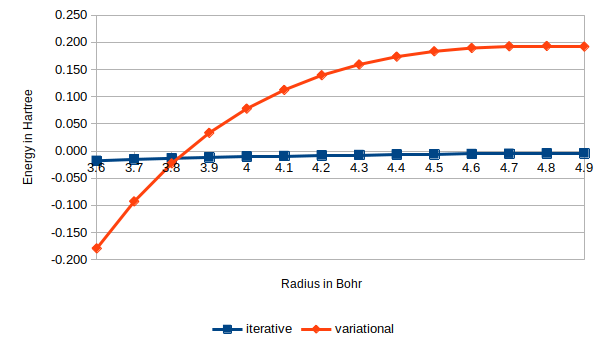
\includegraphics[width=0.75\linewidth]{img/watvarEr.png}
  \caption{Relative difference between the Reaction field energy of \ce{CN^-} in a water solution calculated with \mrchem
  and with different basis sets in Gaussian}
  \label{fig:watvarEr}
\end{figure}

\begin{figure}[h!]
  \centering
  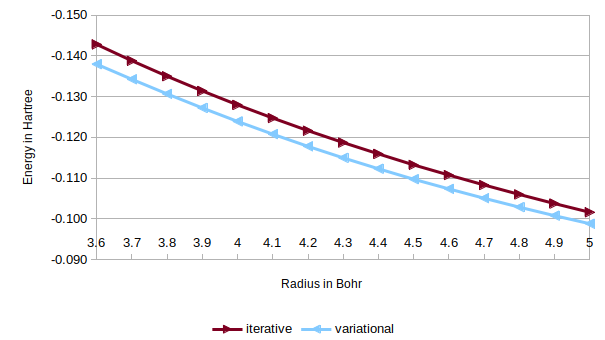
\includegraphics[width=0.75\linewidth]{img/lipvarEr.png}
  \caption{Relative difference between the Reaction field energy of \ce{CN^-} in a water solution calculated with \mrchem
  and with different basis sets in Gaussian}
  \label{fig:lipvarEr}
\end{figure}

\begin{figure}[h!]
  \centering
    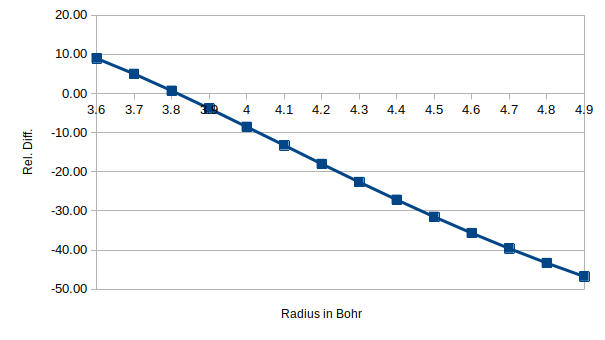
\includegraphics[width=\linewidth]{img/watitervarreldiff.png}
  \caption{Relative difference between the Reaction field energy of \ce{CN^-} in a water solution calculated with \mrchem
  and with different basis sets in Gaussian}
  \label{fig:watreldiffvardaug}
\end{figure}

\begin{figure}[h!]
  \centering
    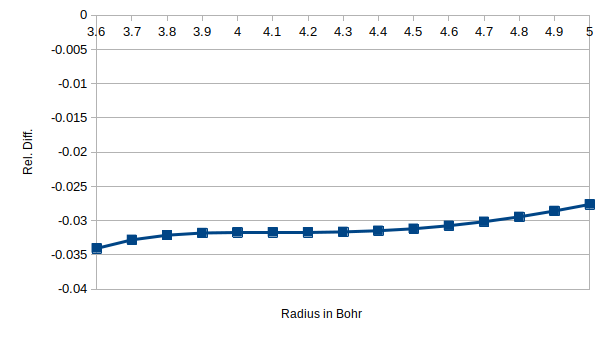
\includegraphics[width=\linewidth]{img/lipitervarreldiff.png}
  \caption{Relative difference between the Reaction field energy of \ce{CN^-} in a water solution calculated with \mrchem
  and with different basis sets in Gaussian}
  \label{fig:lipreldiffvardaug}
\end{figure}



\section{Discussion}
\subsection{Theoretical correctness Discussion}
\subsection{Parametrization Discussion}
The values for water reaction energy with a cavity radius of $5$ Bohr diverged, therefore
we removed them in order to better visualize the trends.
We can see in figures \ref{fig:watreldiffdaug} and \ref{fig:lipreldiffdaug}
that the difference decays the bigger the cavity is. The method Gaussian
uses to calculate the reaction field describes the transition from inside the
cavity to the outside as happening at a boundary, this being the surface of the cavity.
The problem is solved at the surface of the cavity, which is assumed to be extremely
thin, so the transition is noncontinuous, as explained in chapter \ref{chap:Solvent_effect}.
Our cavity is defined as an analytical transition with a parameter $\sigma$ which
controls the width of the the cavity surface, so that we get a smooth transition
between the inside and the outside of the cavity.

Two main factors play that make this decay in relative difference that we observe
a preferred outcome. Firstly the bigger the radius, the smaller the transition is
relative to the size of the cavity. This means that at larger distances our cavity
resembles more and more that of a discontinuous transition such as the ones used
by Gaussian. This means that it is expected that our smooth cavity calculations are expected
to converge to the results of other sharper cavities, such as Gaussian's.

The second factor is the amount of the charge density that is contained within
the cavity. The effect of this can be seen on the tests that followed.

As we can see on the figures \ref{fig:watreldiff02daug} and \ref{fig:lipreldiff02daug}
there is a significant improvement on the relative difference when we compare with
bigger radii of \mrchem calculations to smaller radii of Gaussian calculations.
This is caused by the smooth cavity. Since the transition is wider in our implementation
there is more density that is situated outside the cavity than in cavities of same radius
from Gaussian calculations. This was accounted when we increased the radii, and we still
see the same decay in difference that we saw in the standard comparison.

The graphs from Figure \ref{fig:lipprecreldef} tell us two things about our results:
Firstly at precision lower than $1e-03$ we get results that are at least $20\%$ different
than the best Gaussian results we could run for small radii and diverge from the
Gaussian results for bigger radii. Secondly we see that we don't need a relatively big
precision to get stable results which are consistent with greater previsions and
that also approach the Gaussian results at bigger radii.

On the other hand, it is hard to decide if this is applicable to bigger systems,
as the Lithium cation is fairly simple with a filled energy level, whereas
other systems might not be so simple.

\subsection{Comparison Discussion}
Same as with the tests for \ce{Li^+} and water, the Figures \ref{fig:nopreldiffdaug}
and  \ref{fig:cyanreldiffdaug} show that both relative differences for \ce{CN^-}
and \ce{NO^+} decay at higher radii.

The results for \ce{NO^+}  seem to decay faster than the other molecules, but it
is hard to see due to the lack of data points. Assuming that it decays faster,
one can explain this as being due to the fact that the electron density is
closer to the atoms, making it easier for the cavity to contain most of it.
The opposite can be seen for \ce{CN^-}. The explanation for this might go through
the same line of thought as that for \ce{NO^+}, but now since the molecule is negatively
charged, the density is more diffuse, making it harder to contain it in its entirety.

The divergence around at interval $(4.0, 4.7)$ can be attributed to the way the
functions are projected. The cavity function is very sharp at the transition. In order to
project it correctly one needs to go to very low scales.

Additionally, the intervals are
powers of two, meaning that there is always the discontinuity from the wavelets at the
$4.0$ point, which is hard to correct. This discontinuity brings forth numerical
noise that gets amplified when the derivative of the function is calculated to solve the
\ac{GPE}.

Fosso--Tande defined the derivative of the Cavity as combinations of analytical
derivatives \cite{FossoTande:2013ka}. This definition supposedly would help
remove numerical noise at the transition, since one can create these analytical
derivatives before projecting them into the \ac{MW} basis.

The tables for the \ac{ABC} tests  show us that for most the molecules, the
relative difference doesn't vary too much when going to \ac{ABC} or that it gets
much better, as is the case for \ce{NO^+} in Table \ref{tab:nopabcreldiff}.
It can be seen that, while its single cavity plot, Figure \ref{fig:nopreldiffdaug}, do not go
lower than a relative difference of $10\%$, its \ac{ABC} tests have a relative difference
of less than $4\%$. The same can be said for the results for \ce{CN^-}, in Table \ref{tab:cyanabcreldiff},
which got to less than $3\%$ from the Gaussian results, while it never approached $10\%$
with single cavity, Figure \ref{fig:cyanreldiffdaug}.

The water results, in table \ref{tab:watabcreldiff} do not go too far from the best relative difference
shown in Figure \ref{fig:watreldiffdaug}. They do get slightly better when increasing
the Radius of the interlocking spheres, a decrease in the relative difference of
around $1\%$. This small decrease is seen in the other molecules as well, where,
for \ce{NO^+}, the decrease is around $0.1\%$.

\ce{CH_3CONH_2}, in Table \ref{tab:acetamidabcreldiff} has a difference of at
best $11.4\%$ and at worst $18.6\%$. Increasing the radii of the interlocking spheres
has the same effect that was observed for water.  This tells us that the choice of
radii, the Bondi radii multiplied by a factor of $1.2$, are already a good choice
for the molecules.
\subsection{Variational implementation discussion}
The results for the variational implementation should ideally be the same as the results for the
iterative implementation. From Figures \ref{fig:watreldiffvardaug} and \ref{fig:lipreldiffvardaug}
we can see that this is not the case.
The for this deviation from the results might be because of the same reason the ion
molecules in the comparison tests didn't converge in certain radii. That is, that there
is numerical noise that is being amplified by derivation. Before we had some convergence, since
we still iterated until the potential was converged before optimizing the orbitals. Now
we do not iterate and just calculate the potential once. This might let the numerical errors
be carried over.

A problem with the numerical error explanation is that the differences are still
continuous, that is, it is not nonsense numbers. The reason for this might be that
the way the effective charge distribution $\rho_{eff}$ is implemented, where $\rho_{eff}$
is divided by a function of the cavity. If the cavity diverges and becomes much bigger
than the distribution then $\rho_{eff}$ is essentially zero. This way one might iterate
with only the Surface charge distribution. This can cause the results to not vary
extremely.

If one observes Figure \ref{fig:lipreldiffvardaug} one can see that the difference is not
that big. The difference is at most $3.5\%$ which is not an extremely bad value.
What we can take then is that, although bigger molecules give wrong energies, for smaller
one atom systems, the variational method might be equivalent to the iterative.

\section{Areas of improvement/future development}
Given that the iterative values gave results as expected we can say that the
implementation is correct. An improvement would be to try to change the cavity
definition so as to take into account more of the electron density. One way that is
possible right now is to decrease the width of the transition, another is to simply use
bigger cavities as these are shown to give better results. Both of those are possible
with the implementation used now, but decreasing the width of the transition might
make the cavity harder to project.

A better solution to this is to implement the derivative of the caivty as
a combination of analytical derivatives, as Fosso--Tande did in \cite{FossoTande:2013ka}, which
might let us get better results with the same parameters used in the tests of this chapter.

Another attractive solution is to use layered cavities, in which we have a step-like
cavity transition. Some other methods do that already \cite{Tomasi:2005ipa} although
not with a continuous cavity function.

The goal in the future is to apply these solutions and test if they better the
results of the variational method. After that we will start seeing how molecular properties
are affected by this.



\begin{acronym}
\acro{AUS}[\href{https://www.sigma2.no/content/advanced-user-support}{AUS}]{Numerical Methods in Quantum Chemistry}
\acro{BO}{Born-Oppenheimer}
\acro{CTCC}[\href{http://www.ctcc.no}{CTCC}]{Centre for Theoretical and Computational Chemistry}
\acro{DC}{Dielectric Continuum}
\acro{DFT}{Density Functional Theory}
\acro{EFP}{Effective Fragment Potential}
\acro{EU}{European Union}
\acro{HF}{Hartree-Fock}
\acro{Hylleraas}[\href{https://www.mn.uio.no/hylleraas/english/}{Hylleraas}]{Hylleraas
  Centre for Quantum Molecular Sciences}
\acro{HPC}{High Performance Computing}
\acro{KTH}{Royal Institute of Technology}
\acro{LDA}{Local Density Approximation}
\acro{MCD}{Magnetic Circular Dichroism}
\acro{MCSCF}{Multiconfiguration Self Consistent Field}
\acro{MM}{Molecular Mechanics}
\acro{MW}{Multiwavelet}
\acro{NFR}{Norwegian Research Council}
\acro{NMQC}[\href{http://www.ctcc.no/events/conferences/2015/numeric-conference/}{NMQC}]{Numerical Methods in Quantum Chemistry}
\acro{NOTUR}[\href{https://www.notur.no/}{NOTUR}]{Norwegian Metacenter for Computational Science}
\acro{PCM}{Polarizable Continuum Model}
\acro{PI}{Primcipal Investigator}
\acro{QC}{Quantum Chemistry}
\acro{QM}{Quantum Mechanics}
\acro{QM/MM}{Quantum Mechanics/Molecular Mechanics}
\acro{ROA}{Raman Optical Activity}
\acro{SC}{semiconductor}
\acro{SCF}{Self Consistent Field}
\acro{SHG}{Second Harmonic Genertation}
\acro{STSM}{Short-term scientific mission}
\acro{TPA}{Two-Photon Absorption}
\acro{WP}{Work Package}
\acro{CBS}{Complete Basis Set}
\acro{TCG}{Theoretical Chemistry Group}
\acro{vdW}{van der Waals}
\acro{SE}{Schrödinger Equation}
\acro{PES}{Potential Energy Surface}
\acro{LCAO}{Linear Combination of Atomic Orbitals}
\acro{MRA}{Multi-Resolution Analysis}
\acro{NS}{Nonstandard}
\end{acronym}

\biblio
\end{document}
